%%%%%%%%%-----------------------------------------------------------------
%%%%%%%%% Thesis template, v1
%%%%%%%%% Mathematical & Statistical Methods group - Biometris
%%%%%%%%% Wageningen University & Research
%%%%%%%%%-----------------------------------------------------------------


\documentclass{amsart}

\usepackage{booktabs}
\usepackage{lipsum}

% Setting margins
\usepackage[a4paper, left=3cm,right=3cm]{geometry}

% Packages for the titlepage
\usepackage{tikz}
\usetikzlibrary{calc}
\usepackage{graphicx}
\usepackage{newtxtext}
\usepackage{float}
\usepackage{svg}

% Packages for mathematical writing
\usepackage{amsmath}                           % Enables the align enviroment
\usepackage{amssymb}                           % Math symbols (e.g. \mathbb{})
\usepackage{dsfont} 	                         % For \mathds{1} blackboard bold 1
\usepackage{bm}                                % For roman (upright) bold latin letters
\usepackage{mathtools}                         % Better math
\usepackage[hypertexnames=false]{hyperref}     % For urls and hyperlinks
\usepackage[scientific-notation=true]{siunitx} % For scientific notation
\usepackage{euscript}[mathcal]
\usepackage{txfonts}

% For theorems, remarks, lemmas etc.
\usepackage{amsthm}
\theoremstyle{plain}
\newtheorem{theorem}{Theorem}%[section]
%% >> Define your newtheorems here

% For algorithms
\usepackage[ruled,vlined]{algorithm2e}
\usepackage{algpseudocode}
\renewcommand{\algorithmicrequire}{\textbf{Input:}}
\renewcommand{\algorithmicensure}{\textbf{Output:}}

% Often used math operators:
% You can define these yourself using \DeclareMathOperator and \newcommand
%\DeclareMathOperator*{\argmax}{arg\,max}    % maxmizing argument
%\newcommand{\LA}{\mathbf{\Lambda}}

% For bibliography
\usepackage[
    backend=biber,
    style=ieee, 
    maxcitenames=1,
    mincitenames=1]
    {biblatex}
\addbibresource{references.bib}
\def\bibfont{\footnotesize}


%--------------------------------------------------------------------
%--------------- Front and Main matter style ------------------------
\newcommand{\frontmatter}{
    \pagenumbering{roman}   % Setting page numbering to lower-case roman
}
\newcommand{\mainmatter}{
    \newpage
    \pagenumbering{arabic}  % Setting page numbering to normal integers
}
%--------------- Front and Main matter style ------------------------
%--------------------------------------------------------------------


\begin{document}
% \Sconcordance{concordance:Thesis_Template_Biometris.tex:Thesis_Template_Biometris.rnw:1 %
65 1 1 0 345 1 1 9 11 0 1 2 136 1}



% Add title page:
%------------------------------------------------------------------------------
% In this segment, enter the desired student data to be shown at the title page
\newcommand{\thesisAuthor}{George Miliarakis}                             % State your name
\newcommand{\thesisTitle}{Mechanistic links between ApoE genotype and serum metabolites in Alzheimer's Disease}                                      % State title thesis
\newcommand{\thesisSubTitle}{a Data Science approach}                            % State subtitle thesis
\newcommand{\thesisDegree}{MSc Thesis}      % Choose type
\newcommand{\university}{Wageningen University \& Research}                % You generally don't need to touch this
\newcommand{\thesisPlaceDate}{Wageningen, November 2023}                      % State month and year
%------------------------------------------------------------------------------


%------------------------------------------------------------------------------
% In this segment, enter the desired supervisor data to be shown at the title page
\newcommand{\supervisor}{C.F.W. Peeters}                                                % State name of supervisor
\newcommand{\departmentSUP}{Mathematical \& Statistical Methods (Biometris)} % State department supervisor (generally Biometris)
\newcommand{\universitySUP}{Wageningen University \& Research}                              % State university supervisor (generally WUR)
%------------------------------------------------------------------------------


%------------------------------------------------------------------------------
% In this segment, enter the desired co-supervisor data to be shown at the title page
\newcommand{\cosupervisor}{Yannick Vermeiren}                                         % State name of co-supervisor
\newcommand{\departmentCOSUP}{Nutrition, Brain and Cognitive Ageing}                             % State department or division co-supervisor
\newcommand{\universityCOSUP}{Wageningen University \& Research}                              % State university or company co-supervisor
%------------------------------------------------------------------------------


%------------------------------------------------------------------------------
% Logos and visuals
\begin{titlepage}
\thispagestyle{empty}

% Adding logos
\begin{figure} [H]
\vspace{-3cm}
 \centering
\begin{minipage}[t]{.45\linewidth}
  \raggedright
  % Upload and include SLU loggo here:
  \hspace*{-2cm}
\includegraphics[width=\linewidth]{figures/WURlogo.png}

\end{minipage}%
  \begin{minipage}[t]{.45\linewidth}
  \vspace{-2.6cm}
 \raggedleft
%% Inclusion Biometris logo
 \hspace*{+2cm}
\includegraphics[width =.95\textwidth]{figures/biometris_logo.png}

\end{minipage}
\end{figure}

% Bottom/background picture
\begin{tikzpicture}[overlay, remember picture]
\node[anchor=south west,
      xshift=+6.5cm,
      yshift=-0.2cm]
     at (current page.south west)
     {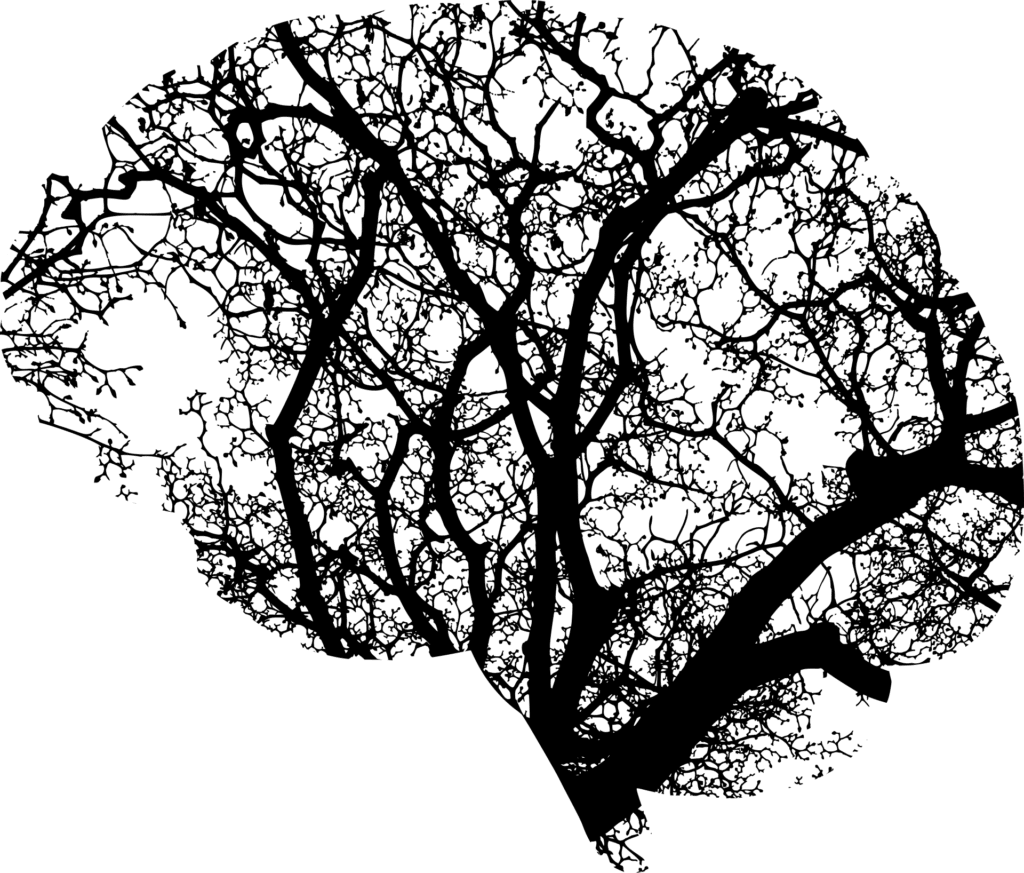
\includegraphics[width = 0.5\textwidth]{figures/torontodeclaration.png}};
\end{tikzpicture}
%------------------------------------------------------------------------------


%------------------------------------------------------------------------------
% Title information
\vspace{1cm}
\begin{center}
\par
\noindent
\rule[0.2cm]{\linewidth}{1.5pt}
\Huge
\textbf{\thesisTitle}
\vspace{0.2cm}
\LARGE
\par
\noindent
\thesisSubTitle\\
\rule[0.2cm]{\linewidth}{1.5pt}
\Large
\end{center}
%------------------------------------------------------------------------------


%------------------------------------------------------------------------------
% Author information
\vspace{2cm}
\noindent
\LARGE
\thesisAuthor\\
\vspace{.2 cm}
\small
\par \noindent
\thesisDegree
\par \noindent
\university
\par \noindent
\thesisPlaceDate
%------------------------------------------------------------------------------


%------------------------------------------------------------------------------
% Supervision information
\vspace{4cm}
\begin{flushright}
\emph{Supervisor} \\
\textbf{\supervisor} \\
\departmentSUP \\
\universitySUP
\end{flushright}

\vspace{.5cm}
\begin{flushright}
\emph{Supervisor} \\
\textbf{\cosupervisor} \\
\departmentCOSUP \\
\universityCOSUP
\end{flushright}
%------------------------------------------------------------------------------


\end{titlepage}

\frontmatter






% Inserting table of contents
\tableofcontents
%--------------- Front matter ---------------------------------------
%--------------------------------------------------------------------






%--------------------------------------------------------------------
%--------------- Main matter ----------------------------------------
\mainmatter

\section{Introduction}\label{Intro}
\subsection{Alzheimer’s Disease}
Alzheimer’s Disease (AD) is a complex, progressive neurodegenerative disorder and the most common form of dementia \cite{Penke2023NewDisease}. It was considered the 6th leading cause of death in the US in 2019, with an overall increase of 145\% in mortality from 2000 to 2019 \cite{20232023Figures}. The impact AD has on patients, their caregivers, and healthcare systems is detrimental. In 2022, caregivers of people with AD or other dementias provided an estimated 18 billion hours of unpaid assistance, valued at \$339.5 billion, more than 14 times the total revenue of McDonald's in 2022 (\$23.3 billion) \cite{20232023Figures}. Its estimated annual global societal cost exceeds the GDP of The Netherlands \cite{Wimo2023The2019}. Despite decades of research, factors to prevent, slow or cure AD remain to be discovered.

The main risk factor for AD is age, while several genetic and lifestyle risk factors, as well as biochemical pathways contribute to its development \cite{Penke2023NewDisease}. AD occurs in various histopathological phenotypes and presents a broad spectrum of clinical signs and symptoms \cite{Heneka2015NeuroinflammationDisease, Edwards2019ANeurodegeneration}. The AD continuum starts with subjective cognitive decline (SCD), followed by mild cognitive impairment (MCI) \cite{Rasmussen2019AlzheimersDiagnosis}, and continues with progressive loss of global cognition, of which particularly memory, processing speed and executive functioning, spanning a total period of 10-15 years \cite{Scheltens2016AlzheimersDisease}. 

The most common phenotype of AD is sporadic or late-onset AD (SAD, LOAD; \>95\% of cases), typically appearing after 65 years of age \cite{Beydoun2014EpidemiologicMeta-analysis}. A rarer phenotype is early-onset familial AD (FAD), usually starting at ages 30–65 and passed in an autosomal dominant fashion \cite{VanCauwenberghe2015ThePerspectives}.
Even though FAD mutations explain only a small percentage of AD cases, they have a great impact on AD research given their appealing genotype-phenotype links.

\subsubsection{Amyloid cascade hypothesis}
The amyloid cascade hypothesis has been the most predominant in explaining the pathogenesis of FAD. In historical terms, its impact was profound, as it helped distinguish and identify AD as a single disease that may be studied for treatment \cite{Hardy2006AlzheimersReappraisal}. It suggests that chronic neuroinflammation promotes protein misfolding and accumulation in the brain, forming plaques (consisting of oligomerized amyloid A$\beta_{42}$) and tangles (consisting of hyperphosphorylated tau protein) \cite{Edwards2019ANeurodegeneration}. Nevertheless, it does not necessarily cover all AD cases; clinical trials of A$\beta$ anti-bodies as treatment prove the amyloid cascade hypothesis insufficient \cite{Kepp2023TheReview,Kurkinen2023TheThinking}. Evidence suggests that oxidative stress, metabolic abnormalities, atherosclerosis, cardiovascular effects, imbalances of intra-neuron calcium and other metal ions contribute to the development of AD \cite{Kepp2023TheReview}. \citeauthor{Kepp2023TheReview} in their recent review propose a more complex and holistic view of AD pathology, by integrating (epi-)genetic, environmental, vascular, neuro-inflammatory and metabolic factors in predictive models \cite{Kepp2023TheReview}. The present study focuses on LOAD patients, integrating and linking genetic and peripheral metabolic nuances in AD.

\subsection{Human apolipoprotein-E gene}
The gene that encodes apolipoprotein-E (ApoE) is the only gene consistently shown associated with LOAD \cite{Corder1993GeneFamilies}.

\subsubsection{ApoE polymorphism is the strongest genetic risk factor for AD}
Humans present three variants of the ApoE gene: $\varepsilon_2$, $\varepsilon_3$ and $\varepsilon_4$ \cite{Husain2021APOETherapeutics, Yang2023ApolipoproteinDisease}, resulting in six genotypes [Fig. \ref{fig1}]. In Caucasian populations apo$\varepsilon_3$ (rs7412 C/rs429358 T) is the most abundant, with a frequency of 78\%, and is considered neutral regarding the risk of AD \cite{Liu2013ApolipoproteinTherapy}. Apo$\varepsilon_4$ (rs7412 C/rs429358 C) has a frequency of 14\% and represents the strongest genetic risk factor for LOAD, in a gene dose-dependent manner \cite{Strittmatter1993ApolipoproteinDisease}. Conversely, apo$\varepsilon_2$ (rs7412 T/rs429358 T) is found in 8\% of Caucasian populations, and carriers of this allele exhibit a reduced risk of LOAD \cite{Liu2013ApolipoproteinTherapy}. The various ApoE alleles are strongly linked to the primary pathological features of LOAD, namely amyloid-A$\beta$ and phosphorylated tau \cite{Deming2017Genome-wideModifiers}. While the association between APOE alleles and LOAD risk or protection is observed across diverse ancestral backgrounds, the strength of this association varies \cite{Belloy2019AForward, Farrer1997EffectsMeta-analysis}.

\begin{figure}[]
  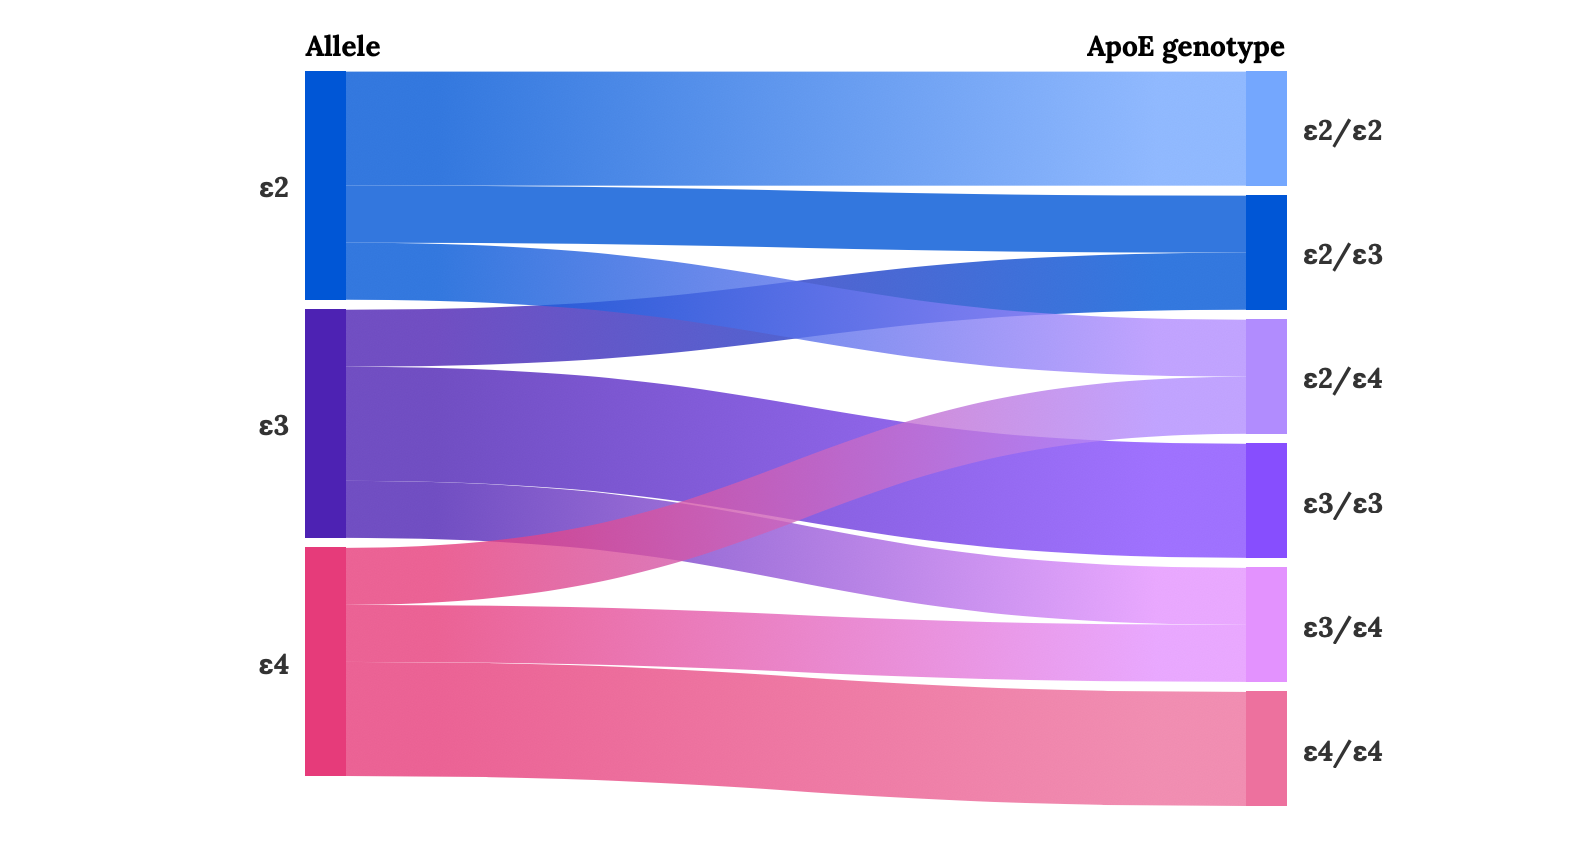
\includegraphics[width=0.7\textwidth]{figures/ApoE@2x.png}
    \caption{Sankey chart showing the allele distribution among the 6 ApoE genotypes.}
  \label{fig1}
\end{figure}

\subsubsection{ApoE and ancestry in AD}
The majority of studies exploring the relationship between ApoE alleles and the genetics of LOAD have primarily focused on Northern European populations\cite{Yang2023ApolipoproteinDisease}. However, smaller investigations involving diverse ancestral backgrounds indicate variations in ApoE4 allele frequencies across different populations\cite{Yang2023ApolipoproteinDisease}. While ApoE4 is present in 14\% of Caucasian Americans, its prevalence increases to 40\% among African Americans, 37\% in Oceania, and 26\% in Australia. Southern Asia and Europe exhibit ApoE4 allelic frequencies of <10\%, contrasting with Northern Europe where it rises to 25\% \cite{Belloy2019AForward, Egert2012ApoEFactors, Eisenberg2010WorldwideHistory, Logue2011AAmericans}.

The epidemiological impact of ApoE alleles also differs among populations. In Korea, Japan, and Japanese-American communities, ApoE4 confers a higher risk of LOAD compared to Caucasians \cite{Farrer1997EffectsMeta-analysis}. Conversely, for Native Americans, Hispanic Americans, African Americans, and those of African descent, APOE4 is associated with a lower risk of LOAD than in Caucasian-American populations \cite{Farrer1997EffectsMeta-analysis, Blue2019LocalHispanics, Suchy-Dicey2022APOEStudy, Rajabli2018AncestralPopulations, Naslavsky2022GlobalSample}. A recent study in a Chinese population found that ApoE3 is more protective than ApoE2 \cite{Chen2011ApolipoproteinDisease}. Some of these population-specific effects are attributed to the ApoE haplotype \cite{Blue2019LocalHispanics, Rajabli2018AncestralPopulations}. A recent discovery of a novel locus (19q13.31) could contribute to attenuating ApoE4-mediated AD risk in African Americans \cite{Rajabli2022AAncestry}.

\subsubsection{ApoE and sex in AD}
Notably, sex (60\% females) and ApoE4 allelic composition (50\% has at least one $\varepsilon_4$ allele) are the strongest genetic risk factors for SAD \cite{, Arnold2020SexMetabolome}. In this regard, it is shown that the ApoE4 genotype has a larger impact on females, as they present greater impairment of mitochondrial energy production, compared to males \cite{Arnold2020SexMetabolome, Yassine2020APOEDisease}.

\subsubsection{Evolution of ApoE over time}
Interestingly, humans are the only ApoE polymorphic species\cite{Yassine2020APOEDisease}. All other animal species have one ApoE variant, which resembles the human $\varepsilon_3$ allele \cite{Hunsberger2019TheInterventions}. ApoE $\varepsilon_4$ is the oldest human allele, followed by $\varepsilon_3$ and $\varepsilon_2$ \cite{Yassine2020APOEDisease}. In highly infectious environments, with food scarcity and shorter lifespans, $\varepsilon_4$ may be adaptive, reducing mortality \cite{Trumble2017ApolipoproteinBurden}. However, as humans transitioned into modern, less infectious environments, with food abundance and longer life expectancy, $\varepsilon_4$ started to burden the arteries and brain, increasing the risk of diseases related to ageing \cite{Yassine2020APOEDisease}. $\varepsilon_3$ emerged from $\varepsilon_4$ and reflects the shift from a plant-based diet to a meat-based one, where ‘meat-adaptive’ genes were and still are vital to control higher lipid levels \cite{Finch1999TheIsoforms}. 

\subsection{ApoE protein}
ApoE is a brain-specific lipid-binding glycoprotein of 299 amino-acids (34 kDa) that comprises several types of lipoproteins, i.e., chilomicra, IDL and VLDL \cite{Husain2021APOETherapeutics}. Its main function in the brain is the transport of lipids (mainly cholesterol) through membrane receptors \cite{Yang2023ApolipoproteinDisease}. The principal producers of ApoE are hepatocytes in the liver \cite{Mahley2016CentralMetabolism}. In the CNS, ApoE is primarily expressed in glia and astrocytes, which modulate metabolic homeostasis and neuronal communication, followed by microglia, the resident immune cells of the brain \cite{Lanfranco2021ExpressionInflammation}.

\begin{figure}[]
  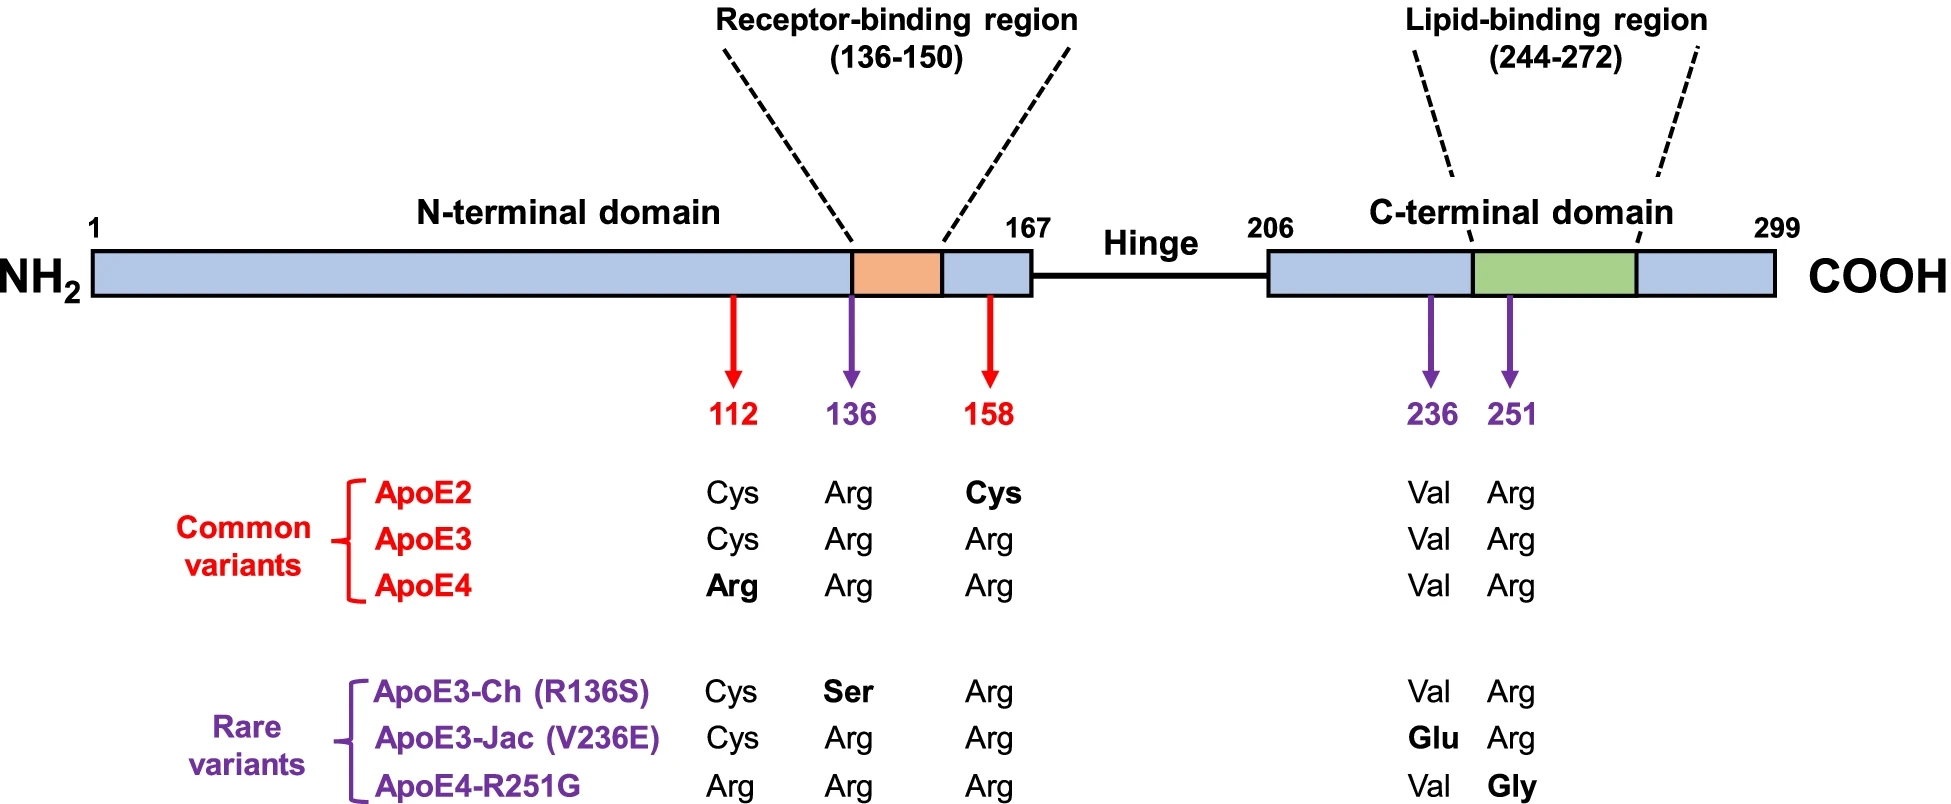
\includegraphics[width=0.7\textwidth]{figures/ApoEprot.png.webp}
    \caption{ApoE protein isoforms.}
  \label{fig2}
\end{figure}

\subsection{Metabolism in AD}

Metabolism entails the repertoire of chemical reactions that keep living organisms alive. Metabolites  --especially lipid \cite{Barupal2019SetsPathophysiology,Fernandez-Calle2022APOEDiseases, Proitsi2017AssociationAnalysis}-- , perceived as functional intermediates of AD development, are rigorously studied for bio-markers or targets for treatment \cite{Oeckl2019ADisease}.

Perturbed serum metabolites associated with AD are amines, aminoacids \cite{deLeeuw2017Blood-basedDisease, Green2023InvestigatingDisease}, cholesteryl esters \cite{Proitsi2017AssociationAnalysis}, sphingolipids \cite{Varma2018BrainStudy,Sun2022AssociationDisease,Green2023InvestigatingDisease,Oeckl2019ADisease,Barupal2019SetsPathophysiology}, fatty acids \cite{Fernandez-Calle2022APOEDiseases,deLeeuw2017Blood-basedDisease}, glycerophospholipids \cite{Varma2018BrainStudy, Jia2022ATypes,Huo2020BrainAnalysis, Weng2019TheImpairment}, phosphatidylcholines \cite{Simpson2016BloodAging} and lipid peroxidation compounds \cite{Fernandez-Calle2022APOEDiseases}. These molecules are usually identified via high-throughput metabolomic pipelines (coupled with Mass Spectrometry (MS) detectors) that trace all compounds in a sample and result in high-dimensional data \cite{Oka2023MultiomicsCohort}. The latter often require advanced statistical methods e.g. projection to latent structures \cite{Weng2019TheImpairment, Peeters2019StableData} or graphical models \cite{Peeters2022Rags2ridges:Matrices} in order to extract putatively meaningful information. 
With such techniques, \citeauthor{deLeeuw2017Blood-basedDisease} discovered distinct serum metabolic signatures among AD patients-controls and those carrying at least one ApoE $\varepsilon_4$ allele \cite{deLeeuw2017Blood-basedDisease}, as they appear in Fig. \ref{fig2}. The different metabolic profiles, however, among ApoE4 non-carriers remain obscure. A data science approach can potentially reveal differentially expressed metabolites between the 6 ApoE genotypes, thus unveiling distinct pathways of metabolic deregulation in AD.

\begin{figure}[b!]
\vspace*{-1cm}
  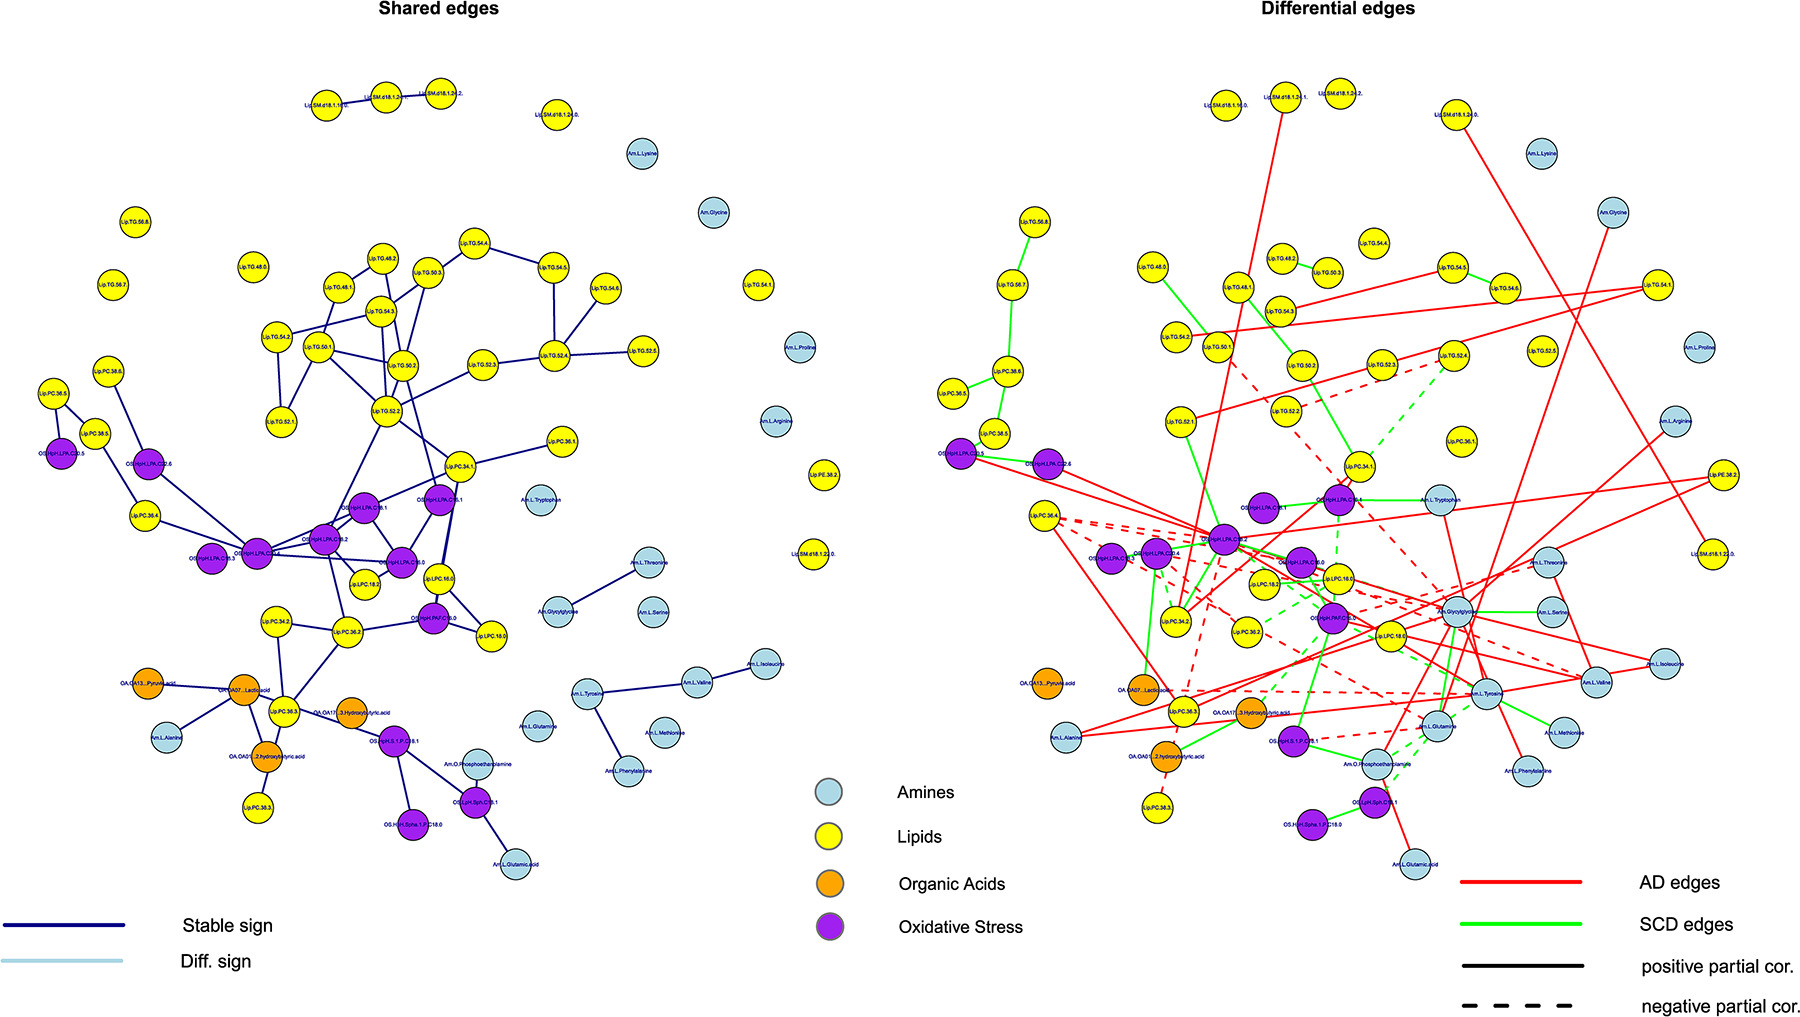
\includegraphics[width=\textwidth]{figures/network.jpeg}
    \caption{Mutual (left-hand panel) and distinct(right-hand panel) metabolic network topologies between ApoE $\varepsilon4$ carriers and non-carriers in AD, as published by \citeauthor{deLeeuw2017Blood-basedDisease}. Red edges represent links that are present exclusively in ApoeE $\varepsilon4$ carriers with AD. Green edges represent connections found in ApoE $\varepsilon4$ non-carriers. Solid edges represent positive partial correlations, while dashed edges represent negative partial correlations. Abbreviations: SCD, subjective cognitive decline }
  \label{fig2}
\end{figure}

\newpage
\subsection{Research Questions}
ApoE $\varepsilon_4$ carriers --particularly females-- experience metabolic disturbances and are at increased risk of SAD. The mechanistic links, however, between ApoE genotype, metabolism and AD development are not entirely known \cite{Fernandez-Calle2022APOEDiseases}, more so among $\varepsilon_4$ non-carriers. Linking specific serum metabolites to distinct ApoE genotypes can reveal metabolic disturbances leading to AD, especially in absence of the ApoE $\varepsilon_4$ allele. Hence, in an effort to elucidate potential links between ApoE genotypes and serum metabolites in AD, one could state the following research questions:

\textbf{RQ}: What are the mechanistic links between ApoE genotype and serum metabolites in AD?
\begin{enumerate}
    \item What is the effect of the ApoE genotype on the expression of serum metabolites?
    \item How discriminatory are serum metabolites among ApoE genotypes?
    \item How do the network topologies of metabolites differ among ApoE genotypes?
\end{enumerate}


\section{Methodology}

\newpage
\subsection{Data management}
The FAIR principles for data management and stewardship in science were published by  ~\citeauthor{Wilkinson2016TheStewardship} in 2016 \cite{Wilkinson2016TheStewardship}. FAIR stands for Findable, Accessible, Interactive, and Reusable data; the intention is to create and use data that are well-documented and reproducible. These principles will be considered at every step of the proposed project and implemented when applicable. All analysis will be performed in R, and the final Thesis report will be written in \LaTeX, as is the current proposal.

\subsection{Analysis}
The degree to which a user can understand and interpret the prediction or decisions made by a statistical model is defined as \textit{interpretability} \cite{Elshawi2019OnHypertension}. It is of interest in this project to find the optimal balance between the performance of a model with its interpretability. The \textit{bias-variance trade-off} was formally introduced by \citeauthor{Geman1992NeuralDilemma} and refers to the trade-off between the accuracy (opposite of bias) and precision (opposite of variance) of a prediction. It also refers to the trade-off between model flexibility (or complexity) and interpretability \cite{Geman1992NeuralDilemma}.
\subsubsection{Differential expression}
A straight-forward way to test whether the metabolites are differentially expressed between the 6 ApoE genotypes is ANOVA (Analysis of Variance) on $p$ linear models. The dependent or response variable in each model would be a metabolite and the independent or explanatory variable would be the ApoE genotype. Let $m_j$ represent the $j$-th metabolite and $G_k$ the $k$-th possible ApoE genotype, an ANOVA model could be:
\[m_j = \mu + G_k +\varepsilon \]
Then, for every $j$ = 1,...,$p$ the hypothesis test would be H$_0$: $G_k=0$ for all $k\in \mathbb{N}, [1,6]$ vs H$_\alpha$: $\exists$ at least one $G_k\neq0$. This implies $p$ hypothesis tests, which creates the problem of multiple testing. A method to treat the latter is controlling False Discovery Rate \cite{Benjamini1995ControllingTesting}, that is controlling the expected ratio of incorrectly rejected hypotheses, globally e.g. at an $\alpha$ of .05.

\subsubsection{Classification}

Considering interpretability, Multinomial Logistic Regression (MNL) is inherently interpretable. Let $y = k$, with $k \in N[1,6]$ representing the k-th ApoE genotype (class) and $\beta_{kj}$ its set of coefficients,  $\beta_{lj}$ the coefficients of the rest of classes for $j$-th metabolite, then an MNL model would calculate the probability

\[\textrm{Pr}(y=k|X=x) =  \dfrac{e^{\sum_{j=1}^{p}\beta_{kj}x_j}}{\sum_{l=1}^{5}\sum_{j=1}^{p}e^{\beta_{lj}x_j}}\]

When $p > n$, the coefficient estimation method has low bias and high variance, in that small changes in the training data can result in very different coefficient estimates \cite{James2023AnEdition}. Regularization trades off a small increase in bias for a great decrease in variance, by shrinking the unimportant coefficients towards zero. LASSO (Least Absolute Shrinkage and Selection Operator) \cite{Tibshiranit1996RegressionLasso}, also called L1-regularization shrinks the MNL coefficients to 0, thus weeding out spurious correlations and reducing the number of predictors \cite{Tibshiranit1996RegressionLasso}. It does so by introducing the term  \[\lambda\sum_{j=1}^{p}|\beta_j|\] where $\lambda \geq 0$ is a tuning parameter that balances the coefficient shrinking effect.

A method to treat collinearity and high dimensionality is a 2-stage Maximum Likelihood(ML) factor analysis (FA), such as the one the package \textbf{FMradio} \cite{Peeters2019StableData} performs. In the 1st stage, a L1-regularised ML estimation is used to filter out redundant features from the data matrix. In the second stage, ML FA projects the aforementioned matrix to an orthogonal space where the features are replaced by -fewer- factors that explain their covariance. One can then use the produced factor scores as predictors in MNL.

Decision Trees (DT) are inherently interpretable, non-parametric models, that fit well large and complicated data sets. They have a tree-like structure that splits the data into branches and leaves(nodes) \cite{Song2015DecisionPrediction}. Random Forests (RF) are ensemble learning methods, that bag several DTs and average their decisions with a majority vote. Despite RFs tend to outperform DTs, they often operate as a \textit{black box} and are poorly interpretable.

The classification performance of the aforementioned models will be holistically assessed using repeated 10-fold CV-obtained AUC (Area Under the ROC curve) and other metrics such as Accuracy, Precision, Recall and F1-score.

\subsubsection{Network analysis}
Network science offers a unifying framework for data and system representation, applicable to any domain \cite{Barabasi2015NetworkScience}. A network, in an abstract sense, consists of nodes connected with links, also referred to as edges. In data science, a network whose nodes represent random features, whose joint probability distribution is defined by the ensemble of their edges is called \textit{graphical model} \cite{Peeters2022Rags2ridges:Matrices}. A \textit{Gaussian graphical model} (GGM) is an undirected graph that represents the conditional independence properties of the features \cite{KollerProbabilisticTechniques}. For instance, let $\mathcal{G=(V,E)}$ be a GGM consisting of a set $\mathcal{V}$ of $p$ vertices, corresponding to random features $Y_1,...,Y_p$ with joint probability distribution $P \sim N_p(\mathbf{0, \Sigma})$, and set of edges $\mathcal{E}$, such that for all pairs $\{Y_i , Y_j\}$ with $i\neq j$:

\[ \mathbf{\Sigma}_{ij}^{-1} = (\mathbf{\Omega}_{ij})=0 \Longleftrightarrow Y_i \Perp Y_j\mid\{Y_k : k \neq i,j\} \Longleftrightarrow (i, j) \notin \mathcal{E} \]

In natural language, a zero value in the inverse covariance matrix (usually referred to as precision matrix $\mathbf{\Omega}$) mutually implies that the respective random features are independent, given the rest of features, which mutually implies that the corresponding features are not connected by an undirected edge $((i, j) \notin \mathcal{E})$ \cite{Peeters2022Rags2ridges:Matrices}.

Network analysis presents a unique approach to visualise high-dimensional and auto-correlated data. In this study, the package \textbf{rags2ridges} \cite{Peeters2022Rags2ridges:Matrices} may be used to generate the feature covariance matrix, as well as the precision matrix, regularise it and represent it in a GGM --as shown in Fig. \ref{fig2}.

\section{Results}

\section{Discussion}


%--------------- Main matter ----------------------------------------
%--------------------------------------------------------------------




%--------------------------------------------------------------------
%--------------- References -----------------------------------------
\newpage
\printbibliography
%--------------- References -----------------------------------------
%--------------------------------------------------------------------







\end{document}



% This is a template for a thesis at Biometris created by C.F.W. Peeters in 2021 
